\documentclass[UTF8]{ctexart}
\CTEXsetup[format={\Large\bfseries}]{section}
\usepackage{amssymb}
\usepackage{amsmath}
\usepackage{cases}
\usepackage{ulem}
\usepackage{geometry}
\usepackage{multirow}
\usepackage{graphicx}
\usepackage{diagbox}
\usepackage{amssymb}
\usepackage{amsmath}
\usepackage{cases}
\usepackage{ulem}
\usepackage[colorlinks,linkcolor=blue]{hyperref}
\usepackage{enumerate}
\usepackage{listings}
\usepackage{color}
\definecolor{dkgreen}{rgb}{0,0.6,0}
\definecolor{gray}{rgb}{0.5,0.5,0.5}
\definecolor{mauve}{rgb}{0.58,0,0.82}
\usepackage{subfigure}

\lstset{frame=tb,
  language=Python,
  aboveskip=3mm,
  belowskip=3mm,
  showstringspaces=false,
  columns=flexible,
  basicstyle={\small\ttfamily},
  numbers=none,
  numberstyle=\tiny\color{gray},
  keywordstyle=\color{blue},
  commentstyle=\color{dkgreen},
  stringstyle=\color{mauve},
  breaklines=true,
  breakatwhitespace=true,
  tabsize=3
}
%算法包
\usepackage{caption}
\usepackage{algorithm,float}
\usepackage{algorithmic}
\usepackage{blindtext}
% Page header
\usepackage{fancyhdr} % Headers and footers
\pagestyle{fancy} % All pages have headers and footers
\fancyhead{}\renewcommand{\headrulewidth}{0pt} 
%算法input output
\renewcommand{\algorithmicrequire}{\textbf{Input:}} % Use Input in the format of Algorithm
\renewcommand{\algorithmicensure}{\textbf{Output:}} % Use Output in the format of Algorithm
\DeclareMathOperator*{\argminA}{arg\,min} % Jan Hlavacek

\setlength{\parindent}{0em}

\geometry{a4paper,scale=0.8}
\begin{document}
\fancyhead[C]{}
\hrule \medskip % Upper rule
\begin{minipage}{0.295\textwidth} 
\raggedright
\footnotesize
崔子寒 \hfill\\   
MG20330012 \hfill\\
zihancui@smail.nju.edu.cn
\end{minipage}
\begin{minipage}{0.4\textwidth} 
\centering 
\large 
Assignment 4\\ 
\normalsize 
Neural Network, 19/20\\ 
\end{minipage}
\begin{minipage}{0.295\textwidth} 
\raggedleft
\today\hfill\\
\end{minipage}
\medskip\hrule 
\bigskip

\section{环境说明}
\begin{itemize}
    \item 操作系统: MacOS 10.15.7
    \item Python版本: 3.6.10 64-bit
    \item Python项目依赖(相近版本应该也可以运行): 
    \begin{itemize}
        \item[*] numpy==1.18.1
        \item[*] matplotlib==3.1.3
    \end{itemize}
    \item 安装依赖: pip install -r requirements.txt
    \item 运行方法: 
    \begin{lstlisting}[language={}]
usage: main.py [-h] [-lr LEARNING_RATE] [--batch-size BATCH_SIZE]
               [--hidden-size HIDDEN_SIZE] [--max-epoch MAX_EPOCH]

Neural Network Training

optional arguments:
  -h, --help            show this help message and exit
  -lr LEARNING_RATE, --learning-rate LEARNING_RATE
                        learning rate, default 0.001
  --batch-size BATCH_SIZE
                        batch size. should be a multiple of 64. default 64
  --hidden-size HIDDEN_SIZE
                        hidden size. default 48
  --max-epoch MAX_EPOCH
                        max epoch. default 1000

    \end{lstlisting}
\end{itemize}
默认的参数是经过测试的比较好的参数,直接运行\texttt{python main.py}即可。

\section{算法设计}
\subsection{问题分析}
首先我们分析问题,我们需要对一个三维空间中的二维曲面进行拟合。我们已经知道这个曲面的方程描述:
\begin{equation*}
    y = sin(x_1) - cos(x_2), x_1\in [-5,5], x_2\in [-5, 5]
\end{equation*}
那么我们首先需要获取训练数据,最简单的方式就是对曲面进行均匀采样,采样出一些数据点作为训练数据。曲面拟合这个任务是一个回归任务,而且我们直接对原始曲面进行采样是可以保证训练数据和真实数据的分布是完全相同的,因此不需要考虑过拟合的问题,也不需要设置验证集进行验证。我们的目标就是让训练误差最小。

\subsection{网络设计}
\begin{figure}[htbp]
    \centering
    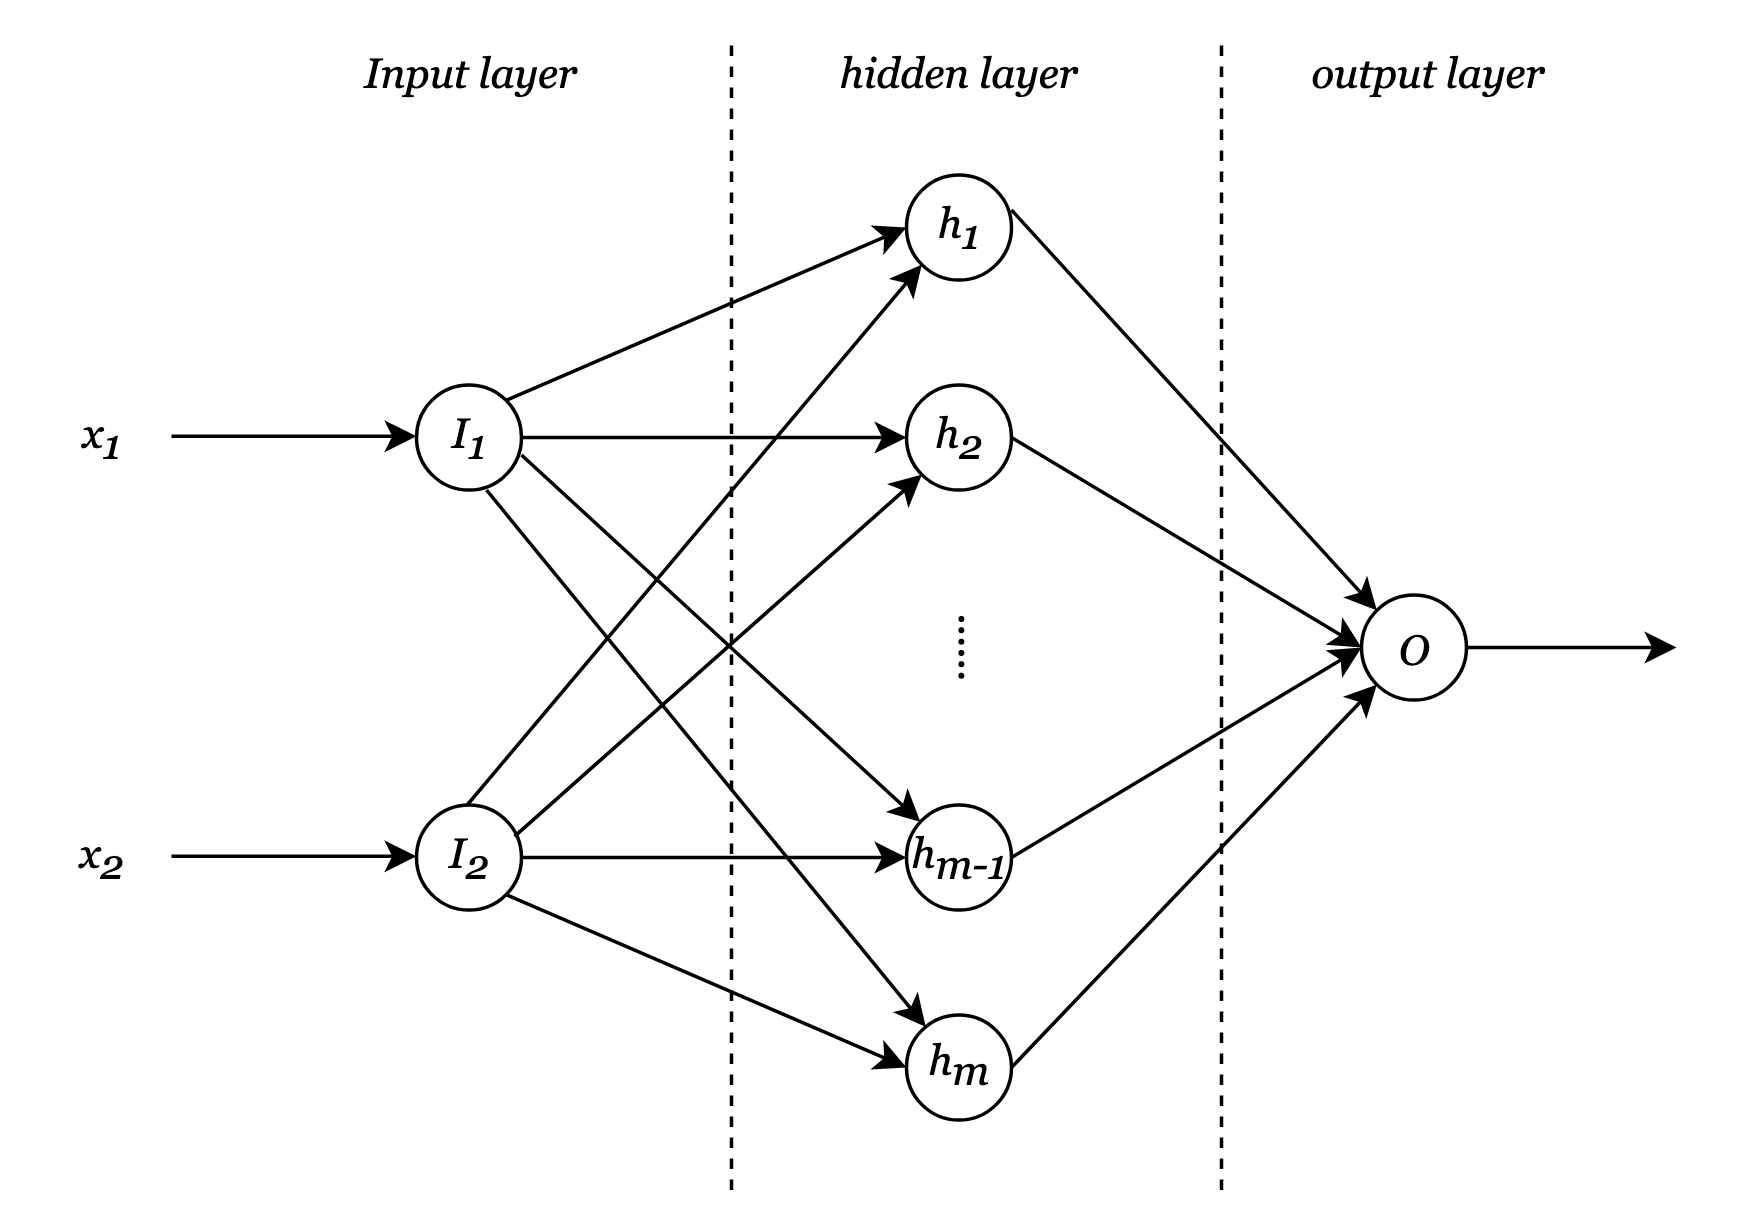
\includegraphics[width=5in]{figures/nn.png}
    \centering
    \caption{网络结构}
\end{figure}

我的网络中使用了单层隐藏层。考虑到曲面拟合是一个比较简单的任务,因此不需要非常深的网络。虽然加深网络提升模型的性能,但是加深网络也会带来问题。网络的深度太大会带来梯度爆炸和梯度消失的问题,也会增加反向传播的计算开销。使用单层隐藏层可以避免这些问题,而且训练较快。但是这需要增加隐藏层的神经元个数,经过测试,至少需要30个以上的神经元才能较好的拟合出给定的曲面,我的实现中使用了48个神经元。

隐藏层的激活函数使用\texttt{sigmoid}函数:
\begin{equation*}
    f(x) = \frac{1}{1+e^{-x}}
\end{equation*}

使用\texttt{sigmoid}函数的原因有:
\begin{itemize}
    \item \texttt{sigmoid}函数非常光滑,便于求导,而且导数的形式简单;
    \item \texttt{sigmoid}函数中有指数部分,可以引入非线性;
\end{itemize}

输出层我们不使用激活函数,直接输出结果。使用均方误差(Mean Squared Error, MSE)来衡量预测值和真实值的差距。
\begin{equation*}
    loss = \frac{1}{m} \sum_{i=1}^m (\hat{y_i}-y_i)^2
\end{equation*}
其中$m$是一个批次的大小(batch size)。
\subsection{算法实现}
\subsubsection{前向传播}
\begin{itemize}
    \item 输入层$\longrightarrow$隐藏层:
    为了加快训练速度,同时也防止单个数据点的梯度太小,我使用批量梯度下降来进行训练。在批量梯度下降中,假定batch size为$m$,那么实际上一个批是一个$m\times 2$大小的矩阵。矩阵的每一行都是一个数据点的坐标$(x_1,x_2)$。假定隐藏层有$l$个神经元,那么对于第$i$个神经元需要训练三个参数,包括两个权重$w_{i1},w_{i2}$和一个偏置$b_i$,但是实际上,可以考虑为输入矩阵新增一列1,那么就可以把$b_i$也看作一个权重,它对应的输入总是1。

    将隐藏层的每个神经元参数当作行向量,构成的矩阵记做$W_{hidden}$,记一个批次的矩阵为$I$,那么隐藏层的输出为:
    \begin{equation*}
        O_{hiddent} = \texttt{sigmoid}(W_{hidden} I^T)
    \end{equation*}
    \item 隐藏层$\longrightarrow$输出层:隐藏层的输出是一个$l\times m$的向量,输出层需要训练的参数是$l$个权值以及一个偏置。记输出层的权值向量为$W_{output}$,,输出层的偏置为$B_{output}$,那么输出层的输出为:
    \begin{equation*}
        O_{output} = W_{output} O_{hiddent}^T + B_{output}
    \end{equation*}

\end{itemize}
\subsubsection{反向传播}
我们使用MSE作为损失函数,那么对于一个批,记它的输出为$\hat{y} = [\hat{y_1},\hat{y_2},\cdots\hat{y_m}]$,记真实值为$y=[y_1,y_2,\cdots y_m]$,那么loss为:
\begin{equation*}
    loss = \frac{1}{m} \sum_{i=1}^m (\hat{y_i}-y_i)^2
\end{equation*}
我们根据权值来分别计算loss关于$B_{output}$,$W_{output}$,$W_{hidden}$的偏导数。
\begin{itemize}
    \item 输出层偏置$B_{output}$:
    \begin{equation*}
        \begin{aligned}
            \frac{\partial loss}{\partial B_{output}} =& \frac{1}{m} \sum_{i=1}^{m} \frac{\partial (\hat{y_i}-y_i)^2}{\partial B_{output}}  \\
            =& \frac{1}{m} \sum_{i=1}^m \frac{\partial (\hat{y_i}-y_i)^2}{\partial \hat{y_i}} \frac{\partial \hat{y_i}}{\partial B_{output}} \\
            =& \frac{2}{m} \sum_{i=1}^m  (\hat{y_i}-y_i) \frac{\partial (W_{output} O_{hiddent} + B_{output})}{\partial B_{output}} \\
            =& \frac{2}{m} \sum_{i=1}^m  (\hat{y_i}-y_i)
        \end{aligned}
    \end{equation*}

    \item 输出层权值$W_{output}$:
    \begin{equation*}
        \begin{aligned}
            \frac{\partial loss}{\partial W_{output}} =& \frac{1}{m} \sum_{i=1}^{m} \frac{\partial (\hat{y_i}-y_i)^2}{\partial W_{output}}  \\
            =& \frac{1}{m} \sum_{i=1}^m \frac{\partial (\hat{y_i}-y_i)^2}{\partial \hat{y_i}} \frac{\partial \hat{y_i}}{\partial W_{output}} \\
            =& \frac{2}{m} \sum_{i=1}^m  (\hat{y_i}-y_i) \frac{\partial (W_{output} O_{hiddent}^T[:,i] + B_{output})}{\partial W_{output}} \\
            =& \frac{2}{m} \sum_{i=1}^m  (\hat{y_i}-y_i) O_{hidden}^T[:,i] \\
            =& \frac{2}{m} (\hat{y}-y) O_{hidden}^T
        \end{aligned}
    \end{equation*}

    \item 隐藏层权值$W_{hidden}$:
    \begin{equation*}
        \begin{aligned}
            \frac{\partial loss}{\partial W_{hidden}} =& \frac{1}{m} \sum_{i=1}^{m} \frac{\partial (\hat{y_i}-y_i)^2}{\partial W_{hidden}}  \\
            =& \frac{1}{m} \sum_{i=1}^m \frac{\partial (\hat{y_i}-y_i)^2}{\partial \hat{y_i}} \frac{\partial \hat{y_i}}{\partial W_{hidden}} \\
            =& \frac{2}{m} \sum_{i=1}^m  (\hat{y_i}-y_i) \frac{\partial (W_{output} O_{hiddent}^T[:,i] + B_{output})}{\partial W_{hidden}} \\
            =& \frac{2}{m} \sum_{i=1}^m  (\hat{y_i}-y_i) \frac{\partial (W_{output} O_{hiddent}^T[:,i] + B_{output})}{\partial O_{hiddent}^T[:,i]} \frac{\partial O_{hiddent}^T[:,i]}{\partial W_{hidden}} \\
            =&  \frac{2}{m} \sum_{i=1}^m  (\hat{y_i}-y_i) W_{output} \frac{\partial \texttt{sigmoid}(W_{hidden}I_i)}{\partial W_{hidden}} \\
            =& \frac{2}{m} \texttt{sigmoid}(W_{hidden}I)*(1-\texttt{sigmoid}(W_{hidden}I)) * (W_{output}(\hat{y}-y)I)
        \end{aligned}
    \end{equation*}
    其中*代表矩阵对应位置元素做乘法。
\end{itemize}

\subsection{代码实现}
当推导出如何计算梯度之后,只需要将参数减去梯度乘上学习率,就可以进行参数更新,具体当代码实现如下:
\begin{lstlisting}[language=Python]
    for epoch in range(self.max_epochs):
            total_error = 0
            if epoch in self.schedule_point:
                print("Decrease lr from {} to {}".format(self.learning_rate, self.gamma * self.learning_rate))
                self.learning_rate *= self.gamma
            for batch in range(len(data_loader)):
                item_X, item_y = data_loader[batch]
                item_X = np.c_[item_X, np.ones(shape=(self.batch_size,1))]
                # forward
                hidden_output = np.dot(item_X, self.hidden_layer.T) # (batch_size, hidden_size)
                output_input = sigmoid(hidden_output)# (batch_size, hidden_size)
                output = np.dot(output_input, self.output_layer).T + self.output_bias# (1, batch_size)
                np.reshape(output, (self.batch_size,)) #(1, batch_size)
                mse_error = np.sum((item_y - output)**2) / self.batch_size
                total_error += mse_error
                
                # backward
                # 输出层偏置
                gradient_output_bias = 2 / self.batch_size
                gradient_output_bias *= np.sum(output-item_y)
                self.output_bias -= self.learning_rate * gradient_output_bias
                
                # 输出层权值
                gradient_output_weight = 2 / self.batch_size
                gradient_output_weight *= np.dot((output-item_y),output_input).T #(hidden_size, 1) 
                self.output_layer -= self.learning_rate * gradient_output_weight
                
                # 隐藏层权值
                gradient_hidden_weight = 2 / self.batch_size
                gradient_hidden_weight *= np.dot(self.output_layer, output-item_y) #(hidden_size, batch_size)
                derivative_activate = (1-output_input) * output_input #(batch_size, hidden_size)
                gradient_hidden_weight *= derivative_activate.T #(hidden_size, batch_size)
                gradient_hidden_weight = np.dot(gradient_hidden_weight, item_X) #(hidden, input_length + 1)
                self.hidden_layer -= self.learning_rate * gradient_hidden_weight
            
            training_loss.append(total_error / len(data_loader))
            print("[Epoch {:>3d}/{}]: MSE Training Loss: {:.8f}.".format(epoch + 1, self.max_epochs, total_error / len(data_loader)))
        return training_loss
\end{lstlisting}

\section{拟合效果}
\subsection{效果展示}
我们使用的训练数据来自对$x_1\in[-6,6],x_2 \in [-6,6]$的均匀采样。测试数据来自于$x_1\in[-5,5],x_2 \in [-5,5]$的均匀采样。
\begin{lstlisting}[language=Python]
import numpy as np
X_train1 = np.linspace(start=-6, stop=6, num=1024)
X_train2 = np.linspace(start=-6, stop=6, num=1024)
X_test1 = np.linspace(start=-5, stop=5, num=1000)
X_test2 = np.linspace(start=-5, stop=5, num=1000)
\end{lstlisting}

我们使用的隐藏层大小为48,Batch size为64,学习率为0.001,在1000个epoch上,训练的效果如下:

\begin{figure}[htbp]
    \centering
    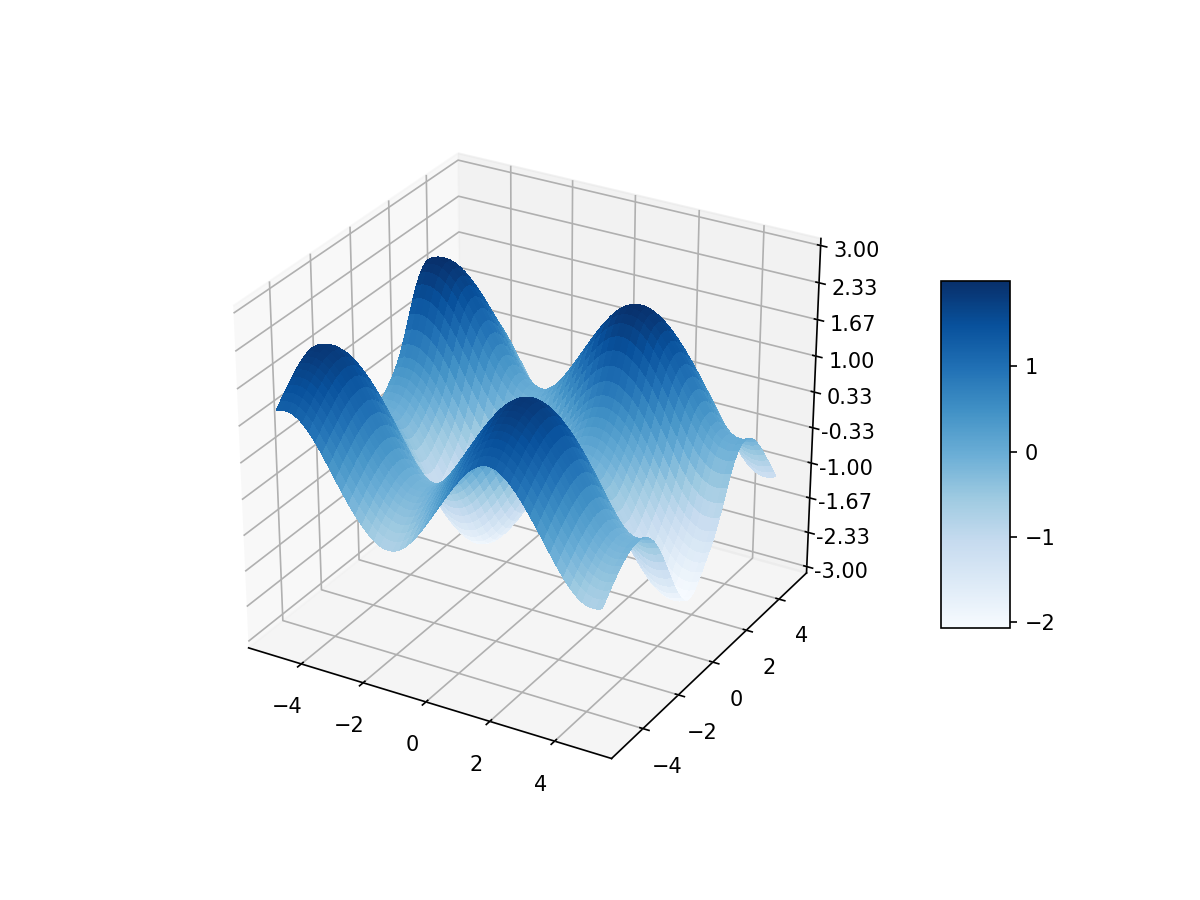
\includegraphics[width=5in]{figures/predict.png}
    \caption{拟合曲面}
    \label{fig:predict}
\end{figure}

\begin{figure}[htbp]
    \centering
    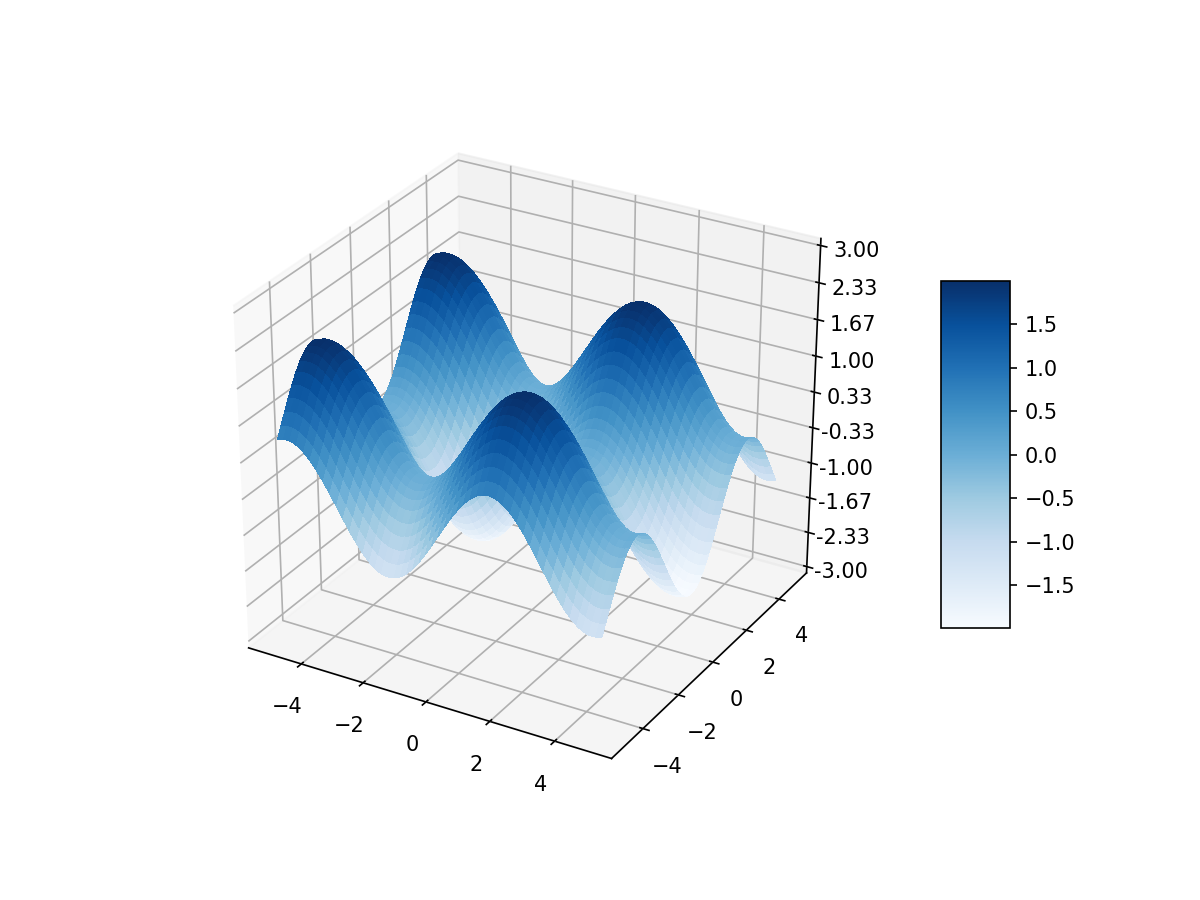
\includegraphics[width=5in]{figures/real.png}
    \caption{真实曲面}
    \label{fig:predict}
\end{figure}

\begin{figure}[htbp]
    \centering
    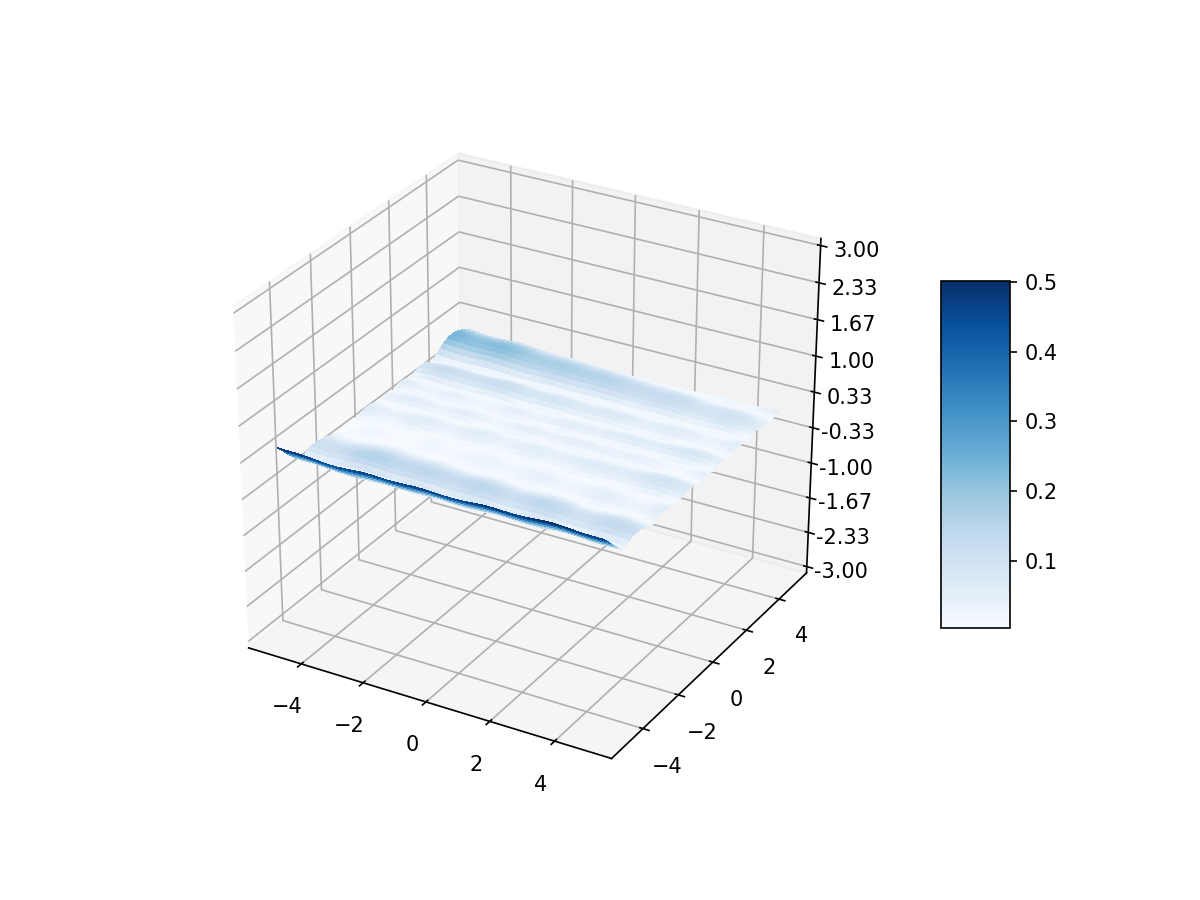
\includegraphics[width=5in]{figures/error.png}
    \caption{误差曲面}
    \label{fig:predict}
\end{figure}

\begin{figure}[htbp]
    \centering
    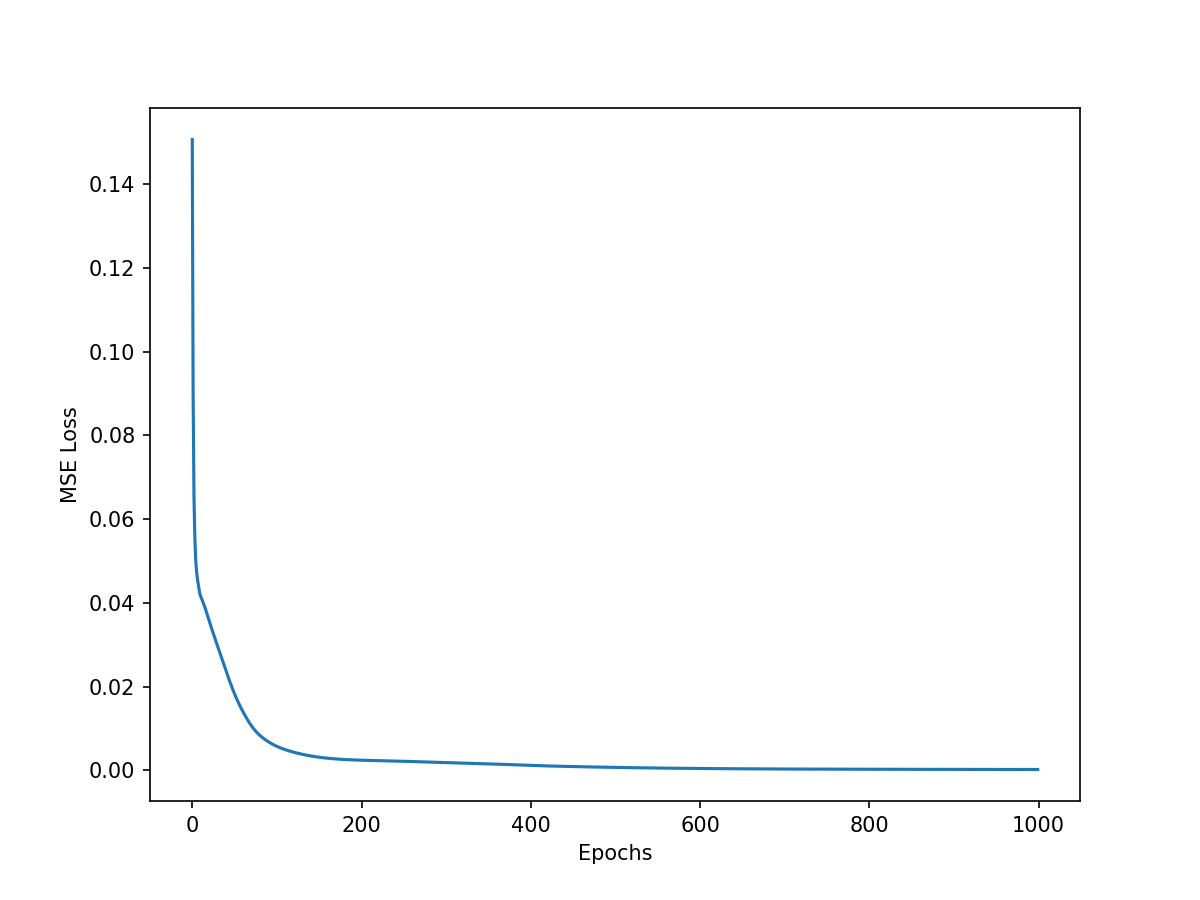
\includegraphics[width=5in]{figures/loss.png}
    \caption{训练Loss曲线}
    \label{fig:predict}
\end{figure}
\subsection{效果分析}
\begin{itemize}
    \item 从Loss上看,网络的训练过程总体稳定,Loss稳步下降,但是由于\texttt{sigmoid}函数会带来的梯度消失的问题,导致训练后期Loss的很慢。
    \item 拟合的曲面较好的反应了真实曲面的特点,最大误差约为0.5。绝大部分数据点的误差在0.1左右。
\end{itemize}


\section{参考}
周志华. (2016). 机器学习. 
\end{document}

